% Springer Nature journal article template (Version 3.1, December 2024)
% Compile with pdfLaTeX and BibTeX in a project containing sn-jnl.cls and
% sn-basic.bst from the official Springer Nature LaTeX template package.
\documentclass[pdflatex,sn-mathphys-num,Numbered]{sn-jnl}

\usepackage{graphicx}
\usepackage{amsmath,amssymb,amsfonts}
\usepackage{booktabs}
\usepackage{braket}
\usepackage{array}
\usepackage{tabularx}
\usepackage{enumitem}
\usepackage{xurl}
\usepackage{etoolbox}

% PDF metadata; hyperref is loaded by the Springer Nature class.
\AtBeginDocument{\hypersetup{
  pdftitle={Factorial Benchmarking of Exact and Finite-Shot Gradient Resolvability in a Four-Qubit Hybrid Quantum Neural Network},
  pdfauthor={Brandon Shen},
  pdfsubject={Factorial benchmarking of exact-gradient signal and finite-shot resolvability in a four-qubit hybrid QNN},
  pdfkeywords={quantum machine learning, quantum neural networks, factorial design, finite-shot gradient estimation, gradient resolvability, reproducible benchmarking}
}}

\urlstyle{same}

% Clean single-author correspondence formatting produced by sn-jnl.cls.
% Keep the conventional author asterisk while avoiding a duplicated asterisk
% on the affiliation, plural labels, and a trailing semicolon after the email.
\makeatletter
\patchcmd{\@maketitle}
  {Corresponding author(s). E-mail(s):}
  {Corresponding author:}
  {}{\PackageWarning{sn-article}{Could not patch corresponding-author label}}
\patchcmd{\email}
  {\textcolor{blue}{#1};\ }
  {\textcolor{blue}{#1}}
  {}{\PackageWarning{sn-article}{Could not remove corresponding-email semicolon}}
\makeatother
\newcommand{\cx}[2]{CX($#1\!\to\!#2$)}
\newcommand{\snrstar}{\mathrm{SNR}^{*}_{\mathrm{est}}}
\newcommand{\snrstark}{\mathrm{SNR}^{*}_{\mathrm{est},k}}
\newcommand{\snrest}{\widehat{\mathrm{SNR}}_{\mathrm{est}}}
\newcommand{\snrestk}{\widehat{\mathrm{SNR}}_{\mathrm{est},k}}
\newcommand{\snrexact}{\mathrm{SNR}_{\mathrm{exact}}}
\newcommand{\vshots}{\mathrm{Var}_{\mathrm{shots}}}

\setlist{nosep,leftmargin=*}
\setlength{\emergencystretch}{1.5em}
\raggedbottom

\begin{document}


\title[Factorial Benchmarking of QNN Gradients]
{Factorial Benchmarking of Exact and Finite-Shot Gradient Resolvability in a Four-Qubit Hybrid Quantum Neural Network}

\author*[1]{\fnm{Brandon} \sur{Shen} (ORCID: \href{https://orcid.org/0009-0002-3545-2106}{0009-0002-3545-2106})} \email{brandonshen123@gmail.com}

\affil[1]{\orgname{Independent Researcher},
\orgaddress{\city{Belmont},
\state{California}, \country{United States}}}

\abstract{Gradient behavior in quantum neural networks depends jointly on circuit structure, objective construction, and finite-shot measurement, yet the interactions among these choices remain incompletely characterized. We study a complete $2^3$ factorial experiment crossing a pair-restricted controlled-NOT (CNOT) schedule ($E$), a normalized transverse-field Ising model (TFIM) energy objective ($L$), and a fixed-gain classical residual shortcut ($R$) in a four-qubit measure--re-encode--reset hybrid quantum neural network. Across 50 matched initialization clusters and 30 finite-shot replicates per scientific cell, we analyze exact-gradient magnitude separately from finite-shot gradient resolvability. The principal finding is a positive $E\times L$ interaction in $\operatorname{asinh}(|g^{\mathrm{exact}}|)$ (centered coefficient $0.004043$; Holm-adjusted $p=0.000739$), supported by an initialization-cluster bootstrap (95\% interval $[0.000473,0.007535]$) and directionally corroborated in an independent-seed dataset. Finite-shot $E\times L$ and $E\times R$ interactions meet the adopted model-based Wald/Holm criterion, but their nested-bootstrap intervals include zero; the residual finding is additionally estimator-mode sensitive. A separately labeled post-audit, 1,000-fit whole-vector bootstrap also leaves the H2--H4 intervals spanning zero; it was not preregistered and does not replace the original analyses. The $L\times R$ interaction moderated by block count remains unresolved. This evidence motivates interaction-aware, measurement-aware QNN benchmarking while characterizing the tested simulation contrasts rather than optimization performance, asymptotic barren-plateau scaling, or hardware-resource advantages.}

\keywords{quantum machine learning, quantum neural networks, factorial design, finite-shot gradient estimation, gradient resolvability, reproducible benchmarking}

\maketitle

\section{Introduction}\label{sec:introduction}

Variational quantum algorithms and quantum neural networks (QNNs) optimize parameterized quantum circuits using objectives defined by quantum-state measurements \cite{cerezo2021vqa,mitarai2018quantum,schuld2019evaluating}. Their gradient behavior can depend on circuit connectivity, observable and objective construction, initialization, and measurement precision. Barren plateaus describe particular regimes of suppressed gradient signal, but initial exact-gradient magnitude is not by itself a measure of finite-shot estimator reliability or successful optimization \cite{mcclean2018barren,anschuetz2022traps,thanasilp2023subtleties,larocca2025barren}.

Prior work has investigated objective locality, entangling structure, initialization, hybrid architectures, and residual pathways \cite{cerezo2021costfunction,ortizmarrero2021entanglement,patti2021entanglement,grant2019identity,skolik2021layerwise,beer2020training,kashif2024resqnets}. Measurement-focused work has shown the importance of observable choice and finite-shot precision \cite{kubler2020adaptive,tamiya2022stochastic,kreplin2024finite,chinzei2025tradeoff,bowles2025backpropagation}. The effects of isolated changes, however, do not automatically determine the interaction between changes when they are combined. This motivates a matched factorial comparison that directly estimates interaction coefficients while distinguishing exact-gradient structure from finite-shot estimator behavior.

We cross three implemented interventions in a four-qubit measure--re-encode--reset hybrid QNN: the within-block CNOT schedule ($E$), the terminal objective ($L$), and a fixed-gain classical shortcut ($R$). All eight combinations are evaluated at matched initial parameter points and hybrid block counts, with defined simulator-shot budgets. The main question is how circuit schedule and objective choice interact in exact-gradient magnitude and whether finite-shot analyses support similarly stable conclusions.

The contributions are threefold. First, we identify a positive centered $E\times L$ interaction in transformed exact-gradient magnitude under the adopted parameter-weighted estimand. Model-based and initialization-cluster bootstrap inference support the result, and an independent-seed analysis retains its positive direction while leaving effect magnitude and block-count dependence uncertain. Second, we distinguish exact-gradient signal from a noisy complete-gradient estimator's plug-in signal-to-noise ratio (SNR), bias, and sign reliability. The H2 and H3 finite-shot interactions satisfy the primary Wald/Holm decision rule but lack nested-bootstrap corroboration; H4 remains unresolved. A later post-audit whole-vector sensitivity likewise retains intervals spanning zero and is reported separately. Third, we provide a reproducible matched $2^3$ factorial benchmark with explicit circuit schedules, reset semantics, measurement-budget accounting, cluster-level inference, and gradient-validation checks. These contributions characterize particular experimental contrasts and provide a methodological example rather than evidence of universal mitigation or optimization advantage.

The published protocol article \cite{shen2026gradient} motivates the adopted factors, model families, hypotheses, transformations, and Holm family, but it reported no data from the present experiment. The current manuscript supplies the complete implemented methodology independently. Operational decisions not fixed in that article, including reset semantics, positive-variance eligibility, and subsequent sensitivity analyses, are distinguished from protocol-derived primary tests in Section~\ref{sec:provenance} and Online Resource~1.

\section{Background and study questions}

\subsection{Finite-sample gradient usability}

For parameter $\theta_k$, let $\hat g_{kr}(\theta)$ be replicate $r$ of the complete finite-shot gradient estimator, $\mu_k=\mathbb{E}_{\mathrm{shots}}[\hat g_{kr}\mid\theta]$, and $\sigma_k^2=\mathrm{Var}_{\mathrm{shots}}[\hat g_{kr}\mid\theta]$. The inaccessible repeated-shot population target is
\[
\snrstark=\frac{|\mu_k|}{\sigma_k}.
\]
With $R_{\mathrm{rep}}=30$ independent finite-shot replicates, the analyzed plug-in estimator is
\[
\snrestk=\frac{|\bar g_k|}{s_k},\qquad
\bar g_k=\frac{1}{30}\sum_{r=1}^{30}\hat g_{kr},\qquad
s_k^2=\frac{1}{29}\sum_{r=1}^{30}(\hat g_{kr}-\bar g_k)^2.
\]
When an exact statevector derivative is available, the complementary measure is
\[
\snrexact(\theta)=
\frac{|g_k^{\mathrm{exact}}(\theta)|}{s_k},
\qquad
\mathrm{Bias}_k(\theta)=\mu_k(\theta)-g_k^{\mathrm{exact}}(\theta).
\]
The plug-in $\snrestk$ compares the estimated mean magnitude with the estimated standard deviation of a \emph{single complete gradient replicate}; it is not the mean-estimate $t$-statistic $\sqrt{30}\,\bar g_k/s_k$. A high value does not establish unbiasedness, correct sign, convergence, or task fidelity. We distinguish population bias $\mu_k-g_k^{\mathrm{exact}}$ from its finite-replicate estimate $\bar g_k-g_k^{\mathrm{exact}}$. Likewise, a plug-in sign comparison based on $\bar g_k$ estimates, but need not equal, population sign agreement based on $\mu_k$. These are complementary estimator diagnostics, not interchangeable definitions of trainability.

H2--H4 analyze $\snrestk$, not $\snrstark$. The plug-in ratio carries finite-replicate uncertainty, motivating resampling of both initialization clusters and within-cell replicates. When $s_k=0$, the mathematical plug-in ratio $|\bar g_k|/s_k$ is undefined if $\bar g_k=0$ and unbounded in the extended-real sense if $\bar g_k\ne0$. The implementation records NaN and positive infinity, respectively; both cases are ineligible for the primary finite-SNR regression analysis, without an epsilon or variance floor. The labeled include-zero sensitivity assigns zero only when both $\bar g_k=0$ and $s_k=0$. Input validation rejects duplicate replicate keys and invalid rows before aggregation; the frozen production validation found neither. Online Resource~1 reports exclusions and conventions in detail.

\subsection{Interventions and interaction hypotheses}

The pair-restricted CNOT factor ($E$) changes the within-block schedule while holding the number of rotations and logical CNOT gates fixed. The objective factor ($L$) replaces global infidelity with normalized TFIM energy; it is a full objective contrast that changes spectral weighting, observable decomposition, measurement requirements, and landscape geometry, not a pure locality intervention. The residual factor ($R$) is a fixed-gain classical shortcut between independently reset quantum blocks and adds no quantum gates or observables.

The novelty claim is intentionally narrow: the individual interventions and metrics are established. To our knowledge, these three implemented contrasts have not previously been evaluated together in a matched factorial experiment that separates exact-gradient magnitude from finite-shot estimator behavior. The strongest prior expectation concerned $E\times L$, because the entangling schedule changes reduced-state derivatives while the objective selects and weights the derivative components entering the measured signal. The published protocol expected sub-additivity at the exact-signal level, but all tests are two-sided \cite{shen2026gradient}.

H1--H4 form one Holm-corrected family at family-wise $\alpha=0.05$:
\begin{itemize}
\item \textbf{H1:} the $E\times L$ coefficient $\eta_{EL}$ in $\operatorname{asinh}(|g^{\mathrm{exact}}|)$ differs from zero;
\item \textbf{H2:} the $E\times L$ coefficient $\beta_{EL}$ in end-to-end $\operatorname{asinh}(\snrest)$ differs from zero;
\item \textbf{H3:} the $E\times R$ coefficient $\beta_{ER}$ differs from zero;
\item \textbf{H4:} the block-count-moderated $L\times R$ coefficient $\beta_{LRD}$ differs from zero.
\end{itemize}
Depth-moderation analyses beyond H4, conditional-estimator analyses, active-residual subset analyses, and configuration-level comparisons are diagnostic or exploratory.

\section{Evaluation protocol and experimental setup}\label{sec:methods}
\subsection{Reference task and objectives}

The reference task is ground-state preparation for the four-site, open-boundary TFIM,
\[
H=-J\sum_{i=0}^{2}Z_i Z_{i+1}-h\sum_{i=0}^{3}X_i,
\qquad J=1,\quad h=0.5.
\]
The target ground state $\ket{\psi_0}$ and eigenvalue bounds $E_0\approx-3.4270$ and $E_{\max}\approx3.4270$ are obtained by exact diagonalization of the $16\times16$ Hamiltonian matrix. Let $\rho_{\mathrm{target}}=\ket{\psi_0}\!\bra{\psi_0}$ and let $\rho(\theta)$ be the prepared state. The global objective is target-state infidelity,
\[
C_{\mathrm{global}}(\theta)
=1-\mathrm{Tr}[\rho_{\mathrm{target}}\rho(\theta)],
\]
and the local objective is normalized TFIM energy,
\[
C_{\mathrm{local}}(\theta)
=\frac{\mathrm{Tr}[H\rho(\theta)]-E_0}{E_{\max}-E_0}.
\]
Both objectives have the same nondegenerate target ground state, preventing target identity from confounding the comparison. The resulting factor still represents the full contrast between normalized TFIM energy and global infidelity, not measurement locality alone: the objectives also differ in spectral weighting, observable decomposition, measurement requirements, and landscape geometry. Prepared-state energy and target fidelity at initialization are therefore reported for every configuration. These are terminal-block prepared-state metrics, not trained or optimized performance.

\subsection{Hybrid block architecture and entangling schedules}
\label{sec:ansatz}

To avoid confusion with objective factor $L$, denote hybrid block count by $D\in\{1,2,3,4,6\}$. Each block independently initializes a four-qubit register to $\rho_{\mathrm{init}}=\ket{0000}\!\bra{0000}$, applies one $R_y$ rotation per qubit followed by four logical CNOTs, and either returns classical features or evaluates the terminal objective. $D$ does not represent uninterrupted coherent circuit depth: only classical information is passed between successive reset blocks. Figure~\ref{fig:architecture} summarizes the architecture.

For block $\ell$, let $x^{(\ell)},\theta^{(\ell)},a^{(\ell)}\in\mathbb{R}^4$ be the classical input, trainable quantum angles, and applied angles, respectively, with $x^{(1)}=\mathbf{0}$. The applied angles and rotation operator are
\begin{equation}\label{eq:angles}
 a_q^{(\ell)}=\theta_q^{(\ell)}+x_q^{(\ell)},\quad
 V_\ell=\bigotimes_{q=0}^3 R_y(a_q^{(\ell)}),\quad
 R_y(a)=e^{-iaY/2}.
\end{equation}
Let $G_{\ell,E,1},\ldots,G_{\ell,E,4}$ be the four CNOT operators in \emph{execution order} according to the schedule below. With matrix products acting right to left,
\begin{equation}\label{eq:unitary}
 U_{\ell,E}=G_{\ell,E,4}G_{\ell,E,3}G_{\ell,E,2}G_{\ell,E,1}V_\ell,\qquad
 \rho_\ell=U_{\ell,E}\rho_{\mathrm{init}}U_{\ell,E}^{\dagger}.
\end{equation}
Here $U_{\ell,E}$ and $\rho_\ell$ are $16\times16$ matrices. No additional activation, clipping, modular wrapping, normalization, rescaling, or encoding gate is applied.

\begin{figure*}[t]
\centering
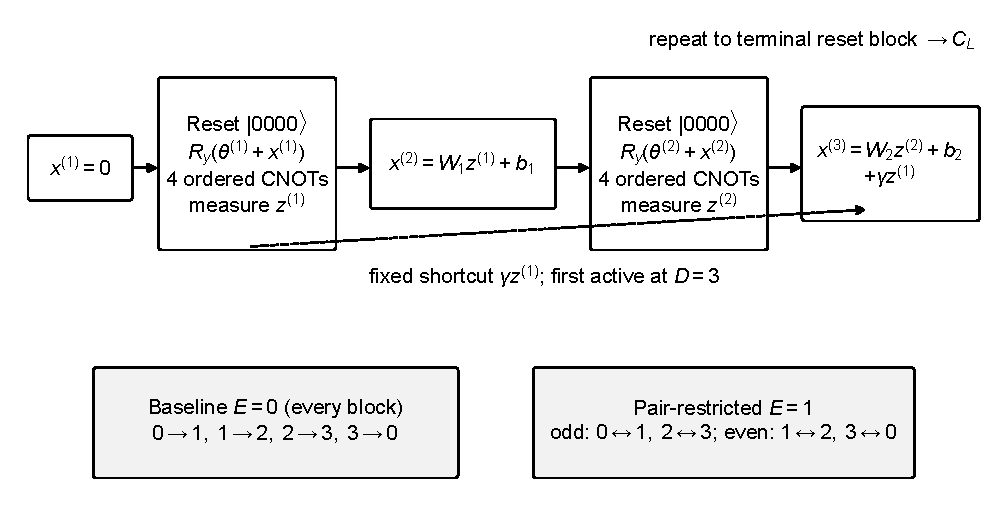
\includegraphics[width=.94\textwidth]{fig16_architecture.pdf}
\caption{Implemented forward pass. Each quantum block starts from a reset four-qubit register, angle-encodes the four-dimensional classical feature by addition to four trainable $R_y$ angles, applies one of the two four-CNOT schedules, and either returns four $Z$ expectations to the classical transition or evaluates the terminal objective. The dashed shortcut is present only for $R=1$ and first changes $x^{(3)}$, so it is inactive for $D=1,2$. The baseline schedule is the ordered ring \cx{0}{1}, \cx{1}{2}, \cx{2}{3}, \cx{3}{0}; the pair-restricted schedule uses the ordered odd/even block pairings stated in the text}
\label{fig:architecture}
\end{figure*}

The schedules each comprise four ordered CNOT gates, keeping logical CNOT count fixed:
\begin{itemize}
\item \textbf{Baseline ($E=0$), every block:} \cx{0}{1}, \cx{1}{2}, \cx{2}{3}, \cx{3}{0}, in precisely that execution order. This is a connected directed ring.
\item \textbf{Pair-restricted ($E=1$), odd blocks $\ell=1,3,\ldots$:} \cx{0}{1}, \cx{2}{3}, \cx{1}{0}, \cx{3}{2}.
\item \textbf{Pair-restricted ($E=1$), even blocks $\ell=2,4,\ldots$:} \cx{1}{2}, \cx{3}{0}, \cx{2}{1}, \cx{0}{3}.
\end{itemize}
Within each restricted block the CNOT operations involve two disjoint qubit pairs; their pairing alternates with block position. No entanglement is carried across blocks, because each block is reset. The connectivity restriction does not imply a universally smaller entanglement entropy or improved optimization performance. The statevector simulator executes gates in the listed order, without transpiler fusion or reordering. Logical gate-count matching is not a claim of equal compiled hardware cost. Because circuit connectivity changes prepared states and their derivatives while the terminal objective determines how those derivatives enter the cost gradient, an $E\times L$ interaction is physically plausible; the experiment does not isolate one universal entanglement mechanism.

\subsection{Residual hybrid architecture}
\label{sec:residual-arch}

For each nonterminal block $\ell<D$, one shared computational-basis measurement setting provides the four features
\begin{equation}\label{eq:features}
 z_j^{(\ell)}=\operatorname{Tr}[(Z_j\otimes I_{\neg j})\rho_\ell],\qquad j=0,\ldots,3,
\end{equation}
where $Z_j\otimes I_{\neg j}$ denotes Pauli $Z$ on qubit $j$ and identity on other qubits (abbreviated $Z_j$ elsewhere). Write $z^{(\ell)}\in\mathbb R^4$, $W_\ell\in\mathbb R^{4\times4}$, and $b_\ell\in\mathbb R^4$. With $z^{(0)}=\mathbf0$, the classical transition is
\begin{equation}\label{eq:transition}
 x^{(\ell+1)}=W_\ell z^{(\ell)}+b_\ell+\gamma z^{(\ell-1)},\qquad
 \gamma=R\in\{0,1\}.
\end{equation}
The fixed residual adds no trainable parameters or quantum gates. The output of each nonterminal block is used only after classical processing, and the next quantum register starts from $\rho_{\mathrm{init}}$. Because $z^{(0)}=0$, the residual first changes a possible real input at $x^{(3)}=W_2z^{(2)}+b_2+\gamma z^{(1)}$. Thus the matched $R=0$ and $R=1$ forward passes are structurally identical when $D\in\{1,2\}$; $D\ge3$ sensitivities are post-primary rather than replacements for the full-sweep H3/H4 models.

The final block $\ell=D$ is evaluated directly with the objective $C_L(\rho_D)$ defined in Section~3.1; it does not produce another inter-block $z^{(D)}$. Equations~\eqref{eq:angles}--\eqref{eq:transition}, the stated CNOT sequences, and the terminal objective completely define the exact-state forward pass. In this mode $z^{(\ell)}$ is evaluated as a statevector expectation; in end-to-end finite-shot mode it is sampled and then re-encoded (Section~\ref{sec:budget}). There are $4D$ quantum rotation parameters and $20(D-1)$ classical weight and bias parameters; H1--H4 analyze only the matched quantum gradients.

Quantum rotation angles are independently initialized from $\mathrm{Uniform}(0,2\pi)$; $W_\ell$ uses Glorot-uniform draws on $[-\sqrt{6/8},\sqrt{6/8}]$ and $b_\ell=0$. For each initialization--$D$ pair, separate quantum and classical streams are derived deterministically from root seed 20260726 using SHA-256. All eight configurations reuse the same initialized arrays and matched parameter indices at fixed initialization and $D$. Distinct block counts use separately derived streams, not shared shallow prefixes. Measurement streams additionally distinguish configuration, estimator mode, budget, and replicate.

\paragraph{Post-audit shot-stream check.}\label{sec:shot-stream-audit}
The shot-seed function reduces its SHA-256-derived value to 31 bits. A complete census found 70 duplicate assignments among 480,000 intended finite-shot vector requests, with no collision within a scientific cell. Nineteen repeated-seed pairs connect two end-to-end vectors; 18 cross initialization clusters treated as independent by the finite-shot inference. Reused seeds do not imply identical measurements: no compared pair had identical complete archived gradient vectors, and individual shot outcomes were not archived. The inferential effect of this cross-cell stream reuse has not been isolated. The vector-preserving bootstrap retains these frozen streams and therefore does not resolve that independence limitation. Initialization matching and the exact-gradient H1 analysis are distinct from this shot-stream issue.

\subsection{Gradient assembly and validation target}

The terminal block's gradient is a direct parameter-shift derivative of the final cost. Every upstream total derivative is assembled by reverse-mode chain rule through the classical maps and quantum-node Jacobians,
\[
\frac{dC}{d\theta_k^{(\ell)}}
=\sum_j
\frac{\partial C}{\partial z_j^{(\ell)}}
\frac{\partial z_j^{(\ell)}}{\partial\theta_k^{(\ell)}}.
\]
Node-level derivatives are evaluated by the two-term parameter-shift rule for Pauli-generated rotations \cite{mitarai2018quantum,schuld2019evaluating}; the downstream sensitivities are propagated exactly through the classical maps. Classical gradients with respect to $W_\ell$ and $b_\ell$ are analyzed separately and are not pooled into the matched quantum-gradient distribution.

The finite-difference audit treats the complete hybrid cost as a black box and compares central finite differences against the assembled total derivative. The audit design is described here; numerical outcomes are summarized in Section~\ref{sec:results-robustness}, with full details in Online Resource 1.

\subsection{Complete factorial design}

All $2^3$ combinations of the binary circuit-schedule ($E$), objective ($L$), and classical-residual ($R$) interventions were evaluated (Table~\ref{tab:configurations}). $E=0$ denotes the ordered ring and $E=1$ the odd/even pair-restricted CNOT sequence; $L=0$ denotes global target-state infidelity and $L=1$ normalized TFIM energy; $R=0$ removes the shortcut and $R=1$ sets its fixed gain to one. Each intervention acts at a different point in the hybrid computation: quantum-state preparation, terminal objective evaluation, or classical propagation. Their joint effects therefore cannot be inferred from comparisons with a baseline alone.

The complete factorial design directly represents main effects and pairwise and three-way non-additivity. In particular, $E\times L$ asks whether the effect of changing the CNOT schedule depends on the chosen objective. The regression coefficient is defined on the adopted transformed-response scale and centered factor coding, not as a universal physical interaction or a raw-gradient difference. All eight configurations share matched initialization arrays and quantum parameter indices within each $D\in\{1,2,3,4,6\}$. Finite-shot comparisons use the same nominal total simulator-shot budgets $B\in\{250,500,1000,2000\}$, but not necessarily the same measurement settings, jobs, or shots per job. The matched gradient distribution contains the $4D$ quantum-rotation derivatives; the $20(D-1)$ classical derivatives are excluded from H1--H4.

\begin{table*}[t]
\centering
\begin{tabular}{cccc l}
\toprule
\# & $E$ & $L$ & $R$ & Description \\
\midrule
1 & 0 & 0 & 0 & Baseline \\
2 & 1 & 0 & 0 & Pair-restricted CNOT schedule only \\
3 & 0 & 1 & 0 & TFIM-energy objective only \\
4 & 0 & 0 & 1 & Residual only \\
5 & 1 & 1 & 0 & $E+L$ combination \\
6 & 1 & 0 & 1 & $E+R$ combination \\
7 & 0 & 1 & 1 & $L+R$ combination \\
8 & 1 & 1 & 1 & All three interventions \\
\bottomrule
\end{tabular}
\caption{Complete $2^3$ factorial design}
\label{tab:configurations}
\end{table*}

\subsection{Finite-shot estimator modes}

Two finite-shot modes are collected; their primary and diagnostic models are analyzed separately:

\begin{itemize}
\item \textbf{End-to-end mode, primary for H2--H4:} forward features and node-level shifted measurements are independently re-estimated in every replicate. Nonlinear downstream re-encoding can therefore induce finite-shot estimator bias.
\item \textbf{Conditional mode, diagnostic:} forward features are held at their exact statevector values while node-level shifted measurements are resampled. This isolates Jacobian-estimation noise from uncertainty caused by re-estimating and re-encoding intermediate features.
\end{itemize}

The conditional mode is not a second primary test and cannot replace an unfavorable end-to-end result. Material disagreement between the modes is interpreted as sensitivity to forward-feature sampling rather than resolved by selecting the more favorable estimator.

For every configuration, block count, initialization, matched quantum-gate parameter, and budget level $B\in\{250,500,1000,2000\}$, the frozen production dataset used 30 independent finite-shot gradient replicates per scientific cell. The analysis included 50 independently initialized top-level design clusters; all other rows are repeated observations. Replicate means, sampling variances, $\snrest$, $\snrexact$, bias, and sign agreement were computed pointwise before aggregation. Cross-cell shot-stream reuse limits finite-shot cluster independence as disclosed in Section~\ref{sec:shot-stream-audit}.

\subsection{Measurement-budget accounting}
\label{sec:budget}

The symbol $B$ denotes the total implemented simulator-shot budget for one replicate's complete gradient vector. The implementation floor-divides $B$ across every required measurement job and distributes the remainder deterministically one shot at a time, so the realized total equals $B$ in every design row. Allocations are nonnegative, deterministic, and give no production job zero shots. This equality does not match circuits, jobs, shots per circuit, physical gates, calibration, readout overhead, hardware noise, or wall-clock time.

For global target infidelity, the simulator draws directly from the exact statevector overlap probability and records one abstract overlap-observable setting. It does not construct an inverse target-state circuit or represent target-state preparation, inverse-preparation gates, or their physical cost. TFIM energy uses one shared Z-basis multinomial setting for the three $ZZ$ terms and one shared X-basis multinomial setting for the four $X$ terms. End-to-end mode additionally samples $D-1$ forward-feature Z jobs and re-encodes their noisy values; conditional mode holds those features exact and intentionally excludes that variance pathway. Primary and conditional diagnostic model inputs are not pooled; the historical descriptive table is qualified below. The implementation records shifted, forward-feature, and objective-observable jobs, settings, and realized shots per job as descriptive resource diagnostics.

\subsection{Primary summaries and estimator-fidelity diagnostics}

The matched quantum-gradient distribution is summarized by the median and interquartile range of pointwise $\snrest$, the fraction of components with $\snrest\ge1$, and dependence on $D$ and $B$. The threshold one is descriptive only: it indicates that the estimator mean equals or exceeds one estimated sampling standard deviation and is not treated as a necessary or sufficient condition for optimization success.

Primary end-to-end models and conditional diagnostic models are separate. The historical \path{results/production_confirmatory/configuration_summaries.csv} instead pooled both finite-shot modes without a mode key and is retained as a labeled historical descriptive artifact. Separately derived post-audit tables are \path{verification/independent_audit/remediation/stage4_20261122_provenance_descriptives/configuration_summaries_finite_shot_end_to_end.csv} and \path{verification/independent_audit/remediation/stage4_20261122_provenance_descriptives/configuration_summaries_finite_shot_conditional.csv}. Their SNR summaries use finite-SNR parameter cells; absolute-bias and empirical sign summaries use all parameter cells. Signed-mean CI fractions inherit explicitly labeled archived CI flags, without a new interval bootstrap. The four historical physics fields were not regenerated in these estimator tables; shared exact-gradient and mode-specific resource references are documented separately. These tables neither replace primary H2--H4 fits nor change their eligibility.

Where exact derivatives are available, the analysis additionally reports $\snrexact$, signed and absolute bias, and
\[
\mathbb{1}\!\left[\begin{gathered}
\bar g_k\ne0,\quad g_k^{\mathrm{exact}}\ne0,\\
\operatorname{sign}(\bar g_k)=\operatorname{sign}(g_k^{\mathrm{exact}})
\end{gathered}\right].
\]
Here $\bar g_k=30^{-1}\sum_{r=1}^{30}\hat g_{kr}$ is the 30-replicate sample mean. The implementation returns false if either the sample mean or the exact derivative is zero, including when both are zero. This is agreement of the sample-mean sign, not a fraction of individual replicate signs. Exact-gradient landscape variance is calculated across matched initializations and remains distinct from repeated-shot variance at fixed parameters.

\subsection{Replicate-count diagnostics and initialization-count provenance}
\label{sec:calibration}

The replicate-count diagnostic used pilot-specific initialization and shot namespaces and began at $R_{\mathrm{rep}}=30$ on representative cells. Its implemented rule checked signed-mean and plug-in-SNR width tolerances, with an explicit stability check only for signed-mean width across increments \cite{davison1997bootstrap,tamiya2022stochastic}. The rule was not met across all representative cells, particularly at shallow block counts; the archived overall return of 200 includes fallback to the search ceiling and does not establish successful uniform calibration. The frozen production dataset retained $R_{\mathrm{rep}}=30$, with no production recollection. These are separately seeded computational precision diagnostics, not evidence that production achieved a uniform prospective calibration. Because $\snrest$ is a plug-in ratio involving an estimated standard deviation, its Monte Carlo uncertainty can remain large after the signed mean is already well resolved.

The archived initialization-count precision calculation used fitted assumptions matching the production end-to-end model. A repository record documents regeneration after the estimator-mode correction; the available files do not establish an independent, excluded initialization-pilot input or the original sample-size decision chronology. Only the candidate $N_{\mathrm{init}}=50$ is recorded, although the configured search increment was 25. Its recorded 90th-percentile simulated Wald 95\% confidence-interval half-widths were below the operational 0.20 threshold for the three then-implemented direct-coded finite-shot interactions. This is a retrospective precision diagnostic, not demonstrated prospective sizing of the corrected centered H1--H4 family; H1 was not evaluated. The threshold is not a smallest effect of interest, equivalence margin, or claim of scientific importance. The production counts are retained as observed design choices, with these provenance and unsuccessful uniform replicate-calibration qualifications.


\subsection{Analysis provenance and amendments}\label{sec:provenance}

The published protocol fixed the eight configurations, block-count and shot-budget sweeps, end-to-end estimator SNR as the primary finite-shot outcome, the mixed-effects model families, H1--H4, the $\operatorname{asinh}$ transformations, and Holm correction \cite{shen2026gradient}. It reported no data from the present implementation and did not fix every operational detail. In particular, its description of the hybrid architecture permits both a reset-per-block reading and a register-persisting reading. We adopted the reset-per-block reading throughout this study (Section~\ref{sec:ansatz}); the alternative would constitute a materially different experiment. The repository preserves the resulting implementation assumptions, decision plans, adjudication records, and verification reports.

An implementation audit found that the originally reported lower-order H1--H3 coefficients had been interpreted using direct 0/1 reference-level coding. The adopted analysis instead uses centered coding, as required for equal averaging over the third binary factor. The direct and centered forms are exact reparameterizations: fitted values, likelihood, residuals, and random effects are unchanged. What changes is the lower-order estimand when a three-way interaction is retained. Historical direct-0/1 H1--H3 values are therefore preserved only as superseded reference-level simple interactions, not as current primary factorial effects. This was an implementation--interpretation correction, not selection of a better-fitting or more favorable model. Positive-variance eligibility, estimator-mode guards, active-residual subset fits, finite-difference checks, and later robustness analyses are labeled separately.

The whole-vector bootstrap and descriptive/provenance corrections described here were performed after the independent audit. They are post-audit sensitivity or documentation work, not protocol-derived primary analyses or preregistered evidence. Original adopted numerical results remain preserved.

\begin{table*}[t]
\centering
\small
\begin{tabularx}{\textwidth}{@{}p{.18\textwidth}p{.25\textwidth}>{\raggedright\arraybackslash}X@{}}
\toprule
Item & Final decision & Interpretive consequence \\
\midrule
Reset semantics & Reset per block & Inference is limited to the implemented measure--re-encode--reset architecture. \\
Factor coding & Centered $\{-1/2,+1/2\}$ & Lower-order pairwise terms average equally over the third binary factor. \\
Residual activation & First active at $D=3$ & Full-sweep H3/H4 estimates include depths at which the residual intervention is inactive. \\
Finite-shot eligibility & Positive replicate variance, $s_k^2>0$ & H2--H4 condition on cells for which the plug-in SNR is defined. \\
Estimator mode & End-to-end primary; conditional diagnostic & The modes are analyzed separately and never pooled. \\
Post-primary checks & Active-depth, cluster-robust, new-seed, and depth-weighting analyses & These analyses assess structural, covariance, seed, and estimand sensitivity without replacing H1--H4. \\
\bottomrule
\end{tabularx}
\caption{Compact analysis-provenance summary. Online Resource~1 gives the complete timing and primary, diagnostic, or post-primary role of each decision and analysis.}
\label{tab:analysis-provenance}
\end{table*}

\subsection{Mixed-effects models}

Let $i$ index initialization, $c$ configuration, $p$ the matched quantum-gate parameter within a block count, $d$ block count, and $b$ shot budget. Binary factors are centered as $E_c=E-1/2$, $L_c=L-1/2$, and $R_c=R-1/2$, each in $\{-1/2,+1/2\}$. Standardized depth is $D_z=(D-3.2)/1.7204650534085253$; 3.2 is the mean of the five tested block counts $D\in\{1,2,3,4,6\}$ and 1.7204650534085253 is their population standard deviation. With the three-way term retained, a lower-order pairwise coefficient averages equally over the third binary factor. Thus H1 and H2 use $E_cL_c$, H3 uses $E_cR_c$ averaged across $L$, and H4 uses $L_cR_cD_z$. Historical direct-0/1 lower-order coefficients instead described simple interactions at the third factor's reference level and are not the adopted primary estimands. The matched repeated-measures structure uses a random intercept $u_i$ for initialization and $v_{idp}$ for matched parameter nested within initialization and block count. The models treat the 50 independently drawn initializations as top-level clusters; all other rows are repeated observations. The finite-shot independence assumption is limited by the cross-cell shot-stream reuse disclosed in Section~\ref{sec:shot-stream-audit}.

For H1, the response is $a_{icpd}=\operatorname{asinh}(|g^{\mathrm{exact}}_{icpd}|)$. The fitted mixed-effects model is
\begin{align}
 a_{icpd}={}&\eta_0+\eta_EE_c+\eta_LL_c+\eta_RR_c
 +\eta_{EL}E_cL_c+\eta_{ER}E_cR_c+\eta_{LR}L_cR_c\nonumber\\
 &+\eta_{ELR}E_cL_cR_c+\eta_DD_{z,d}
 +\eta_{ED}E_cD_{z,d}+\eta_{LD}L_cD_{z,d}+\eta_{RD}R_cD_{z,d}\nonumber\\
 &+u_i+v_{idp}+\epsilon_{icpd}.\label{eq:h1model}
\end{align}
The H1 coefficient $\eta_{EL}$ denotes the modeled $E\times L$ interaction averaged equally across $R$ on the transformed response scale. The adopted pooled model implicitly weights depths in proportion to their $4D$ matched quantum parameters; an equal-depth sensitivity is reported separately. These two weighting conventions target different summaries and should not be conflated.



For H2--H4, the response among positive-variance-eligible cells is $y_{icpdb}=\operatorname{asinh}(\mathrm{SNR}_{\mathrm{est},icpdb})$, and $s_b=\log_2(B_b)$. The protocol-derived model is
\begin{align*}
y_{icpdb}={}&\beta_0
+\beta_E E_c+\beta_L L_c+\beta_R R_c\\
&+\beta_{EL}E_cL_c+\beta_{ER}E_cR_c+\beta_{LR}L_cR_c\\
&+\beta_{ELR}E_cL_cR_c+\beta_DD_{z,d}+\beta_B s_b\\
&+\beta_{ED}E_cD_{z,d}+\beta_{LD}L_cD_{z,d}+\beta_{RD}R_cD_{z,d}\\
&+\beta_{LRD}L_cR_cD_{z,d}
+u_i+v_{idp}+\varepsilon_{icpdb}.
\end{align*}
H2 tests the centered $E_cL_c$ coefficient, H3 the centered $E_cR_c$ coefficient averaged equally over $L$, and H4 the centered $L_cR_c$--depth coefficient. The $E_cL_cR_c$ term is retained. The protocol-derived model uses the full $D$ sweep and is conditional on positive estimated replicate variance. A separate $D\ge3$ fit reports residual-related coefficients as a post-primary sensitivity analysis.

All mixed-effects models are fit in Python 3.12.10 with statsmodels 0.14.6, restricted maximum likelihood (REML), and an L-BFGS-first optimizer fallback order (BFGS, CG, Powell, Nelder--Mead attempted only if L-BFGS fails to converge); no custom convergence tolerances are set beyond each optimizer's library default. A fit is flagged singular if either variance component is within $10^{-8}$ of zero. The original primary and pre-audit sensitivity fits were reported converged and nonsingular; post-audit resampled-fit diagnostics are reported separately in Online Resource~1; an independent BFGS refit of the adopted H2--H4 model gave a maximum absolute difference below $1.12\times10^{-8}$ and a maximum relative difference below $1.20\times10^{-6}$ for the three archived direct-coded finite-shot interaction coefficients; that table alone does not establish the corresponding precision of the centered lower-order contrasts (Section~\ref{sec:results-robustness}). Full package versions, random-seed derivation, and bootstrap sharding are reported in the Software and reproducibility information section below.

\subsection{Inference and multiplicity}

The protocol-derived primary decision rule uses model-based Wald standard errors and two-sided $p$-values. H1--H4 form one family, corrected by the sequential Holm procedure at family-wise $\alpha=0.05$ \cite{holm1979sequential}. Effect estimates, unadjusted confidence intervals, raw $p$-values, and Holm-adjusted $p$-values are all reported; a primary-model rejection requires the adjusted criterion. Failure to reject is not interpreted as equivalence without a prespecified smallest effect of interest and an equivalence test.

The original adopted nested matched bootstrap propagates finite-$R_{\mathrm{rep}}$ uncertainty into coefficient intervals \cite{davison1997bootstrap}. Outer resampling is by complete initialization cluster, retaining all eight configurations, block counts, budgets, and parameter identities. For H2--H4, replicates are independently resampled for each parameter within each selected initialization--configuration--parameter--block-count--budget cell, pointwise SNR is recomputed, and the model is refit. Following the revised stopping instruction, the reported result uses exactly 1,000 unique valid completed nested-bootstrap fits. An additional 178 valid fits completed before workers stopped; these draws are preserved for audit but excluded from the original adopted percentile intervals. H1 uses 2,000 completed initialization-cluster bootstrap fits with zero failures. Bootstrap iterations are distinct from the 50 independent initialization clusters and are not denoted as sample size.

Cumulative checkpoint summaries are reported at 40, 100, 200, 400, 443, and 1,000 completed H2--H4 fits. The 443-fit row is retained as a historical checkpoint rather than the final achieved size. The original adopted percentile endpoints remain finite-Monte-Carlo estimates; order-statistic/binomial-rank intervals quantify Monte Carlo uncertainty in each endpoint separately from scientific sampling uncertainty.

\paragraph{Post-audit vector-preserving sensitivity.}\label{sec:vector-bootstrap-method}
An independent audit identified that the original inner bootstrap sampled parameter components separately even though forward measurements, Jacobian measurements, and reverse-assembled gradients share noise within a complete vector replicate. The separately labeled post-audit sensitivity resampled each complete 30-by-$(4D)$ replicate matrix by rows, sharing each selected replicate index across all quantum parameters within an initialization-copy--configuration--block-count--budget--mode cell. Complete initialization-cluster resampling and distinct copy IDs were retained; different configurations, block counts, budgets, and estimator modes retained separate inner streams. The original SNR definition, per-draw eligibility, fixed-effects model, REML, and random-effects structure were retained. The analysis used a distinct deterministic seed stream and exactly 1,000 accepted fits, excluding diagnostic-pilot draws. It was not preregistered or part of the original primary Holm family, and it does not replace the adopted point estimates, Wald/Holm results, or original percentile intervals. It also retains the frozen shot-stream collisions described in Section~\ref{sec:shot-stream-audit}.


\subsection{Post-run robustness and independent-seed rerun}\label{sec:h2-depth-methods}

Post-primary H1 analyses fit categorical depth moderation separately in the original and independent-seed datasets. Because matched parameter counts grow with depth, observation and matched-parameter weights are identical here: $0.0625$, $0.125$, $0.1875$, $0.25$, and $0.375$ for $D=1,2,3,4,6$. The primary pooled point estimate numerically matches the categorical observation-weighted point estimate; the equal-depth average answers a different question, and differing covariance structures give slightly different standard errors.

Three H1 estimands are distinguished. The retained primary, parameter-weighted estimand is the interaction for a randomly selected implemented quantum parameter among all analyzed parameters; this matches the protocol-derived row-level mixed model and preserves its planned analysis population. The equal-depth estimand is the arithmetic mean of the five categorical depth contrasts, giving each tested $D$ weight $0.2$. Depth-specific estimands are the five separate categorical contrasts. These alternatives diagnose weighting and moderation without replacing the primary coefficient.

Post-primary H3 analyses derived objective-specific $E_c\times R_c$ contrasts at $L=0$ and $L=1$, repeated the fit at active-residual depths $D\in\{3,4,6\}$, tested categorical depth moderation with model-based and initialization-clustered covariance, compared end-to-end and conditional estimator modes without pooling, and performed leave-one-initialization-out diagnostics. These are explanatory or sensitivity analyses, not additions to H1--H4.

Secondary multiplicative indices are conditional on residual status. For the $R=0$ finite-shot comparison shown in Fig.~\ref{fig:el-primary}, let $M_0$, $M_E$, $M_L$, and $M_{EL}$ denote the configuration-level RMS values of pointwise end-to-end $\snrest$ over finite, positive-variance-eligible rows. The corresponding multiplicative interaction index is
\[
I_{EL\mid R=0}
=\frac{M_{EL}M_0}{M_EM_L}.
\]
For exact gradients,
\[
J_{EL\mid R=0}
=\frac{G_{EL}G_0}{G_EG_L},\qquad
J_{EL\mid R=1}
=\frac{G_{ELR}G_R}{G_{ER}G_{LR}}.
\]
Each $G$ follows the frozen configuration-level RMS absolute-exact-gradient construction: unique exact-gradient parameter rows are pooled before aggregation, so deeper block counts receive more parameter/observation weight. Thus $I_{EL\mid R=0}$ summarizes end-to-end finite-shot estimator SNR, whereas the $J$ indices summarize exact-gradient magnitude. These indices are descriptive multiplicative summaries, conditional on $R$, and are not transformations of the centered mixed-model coefficients. Values above one indicate positive departure from the multiplicative no-interaction reference; they are not percentage improvements in optimization. Initialization-cluster percentile intervals for the $J$ indices use 2,000 completed iterations per dataset and residual condition, with zero failures.

Prepared-state task metrics comprise raw TFIM energy, normalized prepared-state energy cost, target fidelity, and target infidelity for the terminal-block state at initialization. Exact-state duplicates across finite-shot budgets are removed. Since $L$ changes the evaluated objective rather than state preparation, paired $L=0$ and $L=1$ summaries are identical when all other factors are fixed. These descriptive metrics are not optimization outcomes.

\subsection{Implementation validation}

The implementation audit included black-box finite-difference validation of assembled hybrid gradients, inspection of reset semantics and residual activation, explicit estimator-mode guards, optimizer refits, deterministic seed checks, and regression testing of all principal analysis paths. Detailed audit history, superseded pooled-mode outputs, bootstrap checkpoints, and script-level provenance are reported in Online Resource 1 and the repository rather than in the main narrative.

\section{Results}

\subsection{Calibration and finite-shot eligibility}\label{sec:results-calibration}\label{sec:zero-variance-sensitivity}

The frozen production dataset used $R_{\mathrm{rep}}=30$ independent gradient replicates per scientific cell and 50 independently initialized top-level design clusters. The replicate-count diagnostic criterion was not met uniformly at shallow block counts, and no production recollection was performed. Exactly zero estimated replicate variance occurred only for $L=0$: 509 of 102,400 end-to-end cells and 1,324 of 102,400 conditional cells, versus none for $L=1$. H2--H4 therefore condition on positive estimated variance; this objective-linked eligibility is retained as a limitation rather than treated as random missingness.

\subsection{Centered exact-gradient interaction (H1)}\label{sec:h1-result}

The corrected centered $E\times L$ exact-gradient interaction was $0.004043$ (SE $0.001081$, Wald 95\% CI $[0.001924,0.006162]$, raw $p=0.000185$, Holm $p=0.000739$). The 2,000-completed-fit initialization-cluster bootstrap had zero failures and a percentile 95\% interval $[0.000473,0.007535]$. H1 is therefore the strongest cross-procedure result.

The new-seed estimate was $0.007726$ (Wald 95\% CI $[0.005592,0.009860]$); its 2,000-fit, zero-failure bootstrap interval was $[0.003402,0.011923]$. This internal seed replication retained the positive direction, but the larger point estimate and depth differences leave magnitude stability uncertain.

Table~\ref{tab:h1-marginal-effects} translates the adopted H1 model into adjusted locations for each objective--schedule combination, averaging equally over residual status and using the adopted parameter/observation weights over depth. On the back-transformed adjusted-location scale, the pair-restricted schedule exceeds the baseline by approximately $0.00230$ under global infidelity and $0.00635$ under TFIM energy, equivalent to approximately 9.9\% and 15.0\% of the respective baseline adjusted locations. The difference between those schedule effects is approximately $0.00405$. These quantities are differences between model-adjusted locations, not arithmetic mean differences in raw gradient magnitudes, and they do not establish improved optimization.

\begin{table*}[t]
\centering
\small
\caption{Model-adjusted H1 marginal predictions and contrasts. Predictions average equally over residual status and use the adopted parameter/observation weights over $D=1,2,3,4,6$. Random effects are set to zero. Original-scale entries are $\sinh$ transforms of adjusted means on the $\operatorname{asinh}(|g_{\mathrm{exact}}|)$ scale and are not arithmetic means of raw gradient magnitudes. The difference in objective-specific schedule effects equals the adopted centered H1 estimand.}
\label{tab:h1-marginal-effects}
\begin{tabularx}{\textwidth}{@{}llXX@{}}
\toprule
\multicolumn{4}{l}{\textbf{Panel A---Adjusted marginal predictions}}\\
Objective & CNOT schedule & Adjusted $\operatorname{asinh}(|g_{\mathrm{exact}}|)$ (95\% CI) & $\sinh$ of adjusted mean (transformed 95\% CI)\\
\midrule
Global infidelity & Baseline & 0.023117 [0.021088, 0.025145] & 0.023119 [0.021090, 0.025148]\\
Global infidelity & Pair-restricted & 0.025413 [0.023385, 0.027442] & 0.025416 [0.023387, 0.027445]\\
TFIM energy & Baseline & 0.042397 [0.040369, 0.044425] & 0.042410 [0.040380, 0.044440]\\
TFIM energy & Pair-restricted & 0.048737 [0.046708, 0.050765] & 0.048756 [0.046725, 0.050787]\\
\midrule
\multicolumn{4}{l}{\textbf{Panel B---Marginal contrasts}}\\
\multicolumn{2}{p{0.30\textwidth}}{Contrast} & Difference on asinh scale (95\% CI) & Difference between $\sinh$-transformed adjusted values (delta-method 95\% CI)\\
\midrule
\multicolumn{2}{p{0.30\textwidth}}{Pair-restricted minus baseline at global infidelity} & 0.002297 [0.000798, 0.003795] & 0.002298 [0.000799, 0.003797]\\
\multicolumn{2}{p{0.30\textwidth}}{Pair-restricted minus baseline at TFIM energy} & 0.006340 [0.004841, 0.007838] & 0.006346 [0.004846, 0.007846]\\
\multicolumn{2}{p{0.30\textwidth}}{Difference in schedule effects, H1} & 0.004043 [0.001924, 0.006162] & 0.004049 [0.001928, 0.006169]\\
\bottomrule
\end{tabularx}
\end{table*}

Post-primary depth contrasts were, for $D=1,2,3,4,6$, respectively, $-0.005251$, $-0.003579$, $0.012588$, $0.004664$, and $0.003446$ in the original data, and $0.001862$, $0.003120$, $0.006250$, $0.007885$, and $0.010870$ in the independent-seed data. The original equal-depth average was $0.002374$ (CI $[-0.000164,0.004911]$), whereas its observation-weighted average was $0.004043$ (CI $[0.001929,0.006157]$). The corresponding independent-seed summaries were $0.005997$ (CI $[0.003443,0.008552]$) and $0.007726$ (CI $[0.005597,0.009854]$). Thus the original equal-depth interval includes zero but the observation-weighted interval does not; both independent-seed intervals exclude zero. Observation and parameter weights are identical. Original depth moderation was detected by the mixed model ($\chi^2(4)=22.844$, $p=0.000136$) but not by initialization-clustered inference ($\chi^2(4)=6.008$, $p=0.1985$). Neither independent-seed test rejected (mixed $p=0.1090$; clustered $p=0.7706$). The depth profile is consequently covariance-sensitive, and the cross-seed magnitude difference has no clear depth localization under the frozen rule.

\begin{figure*}[t]
\centering
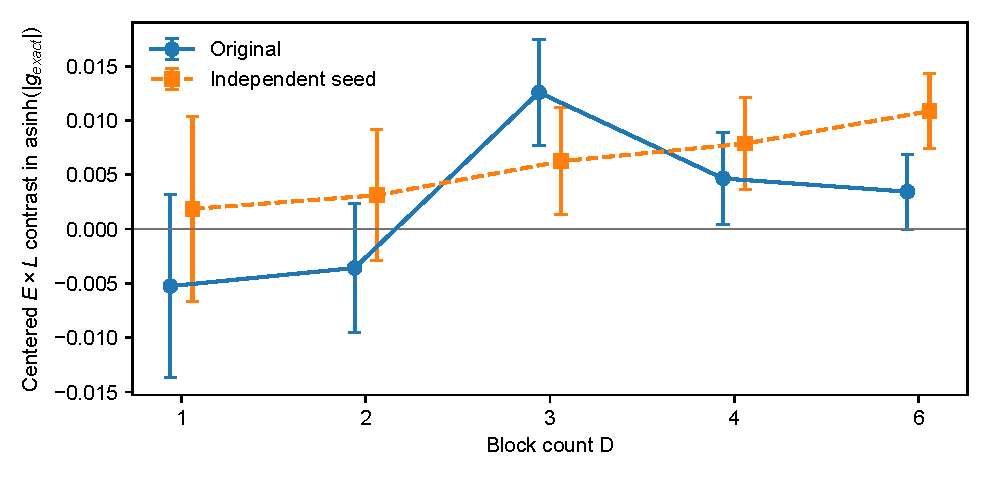
\includegraphics[width=0.78\textwidth]{fig13_h1_depth.pdf}
\caption{Post-primary centered $E\times L$ exact-gradient contrasts by block count in the original and independent-seed datasets. Points show covariance-aware mixed-model contrasts and bars show unadjusted Wald 95\% intervals. Shape and line style distinguish datasets; the horizontal reference is zero. The display does not posit a monotonic depth law}
\label{fig:h1-depth}
\end{figure*}

\begin{figure}[t]
\centering
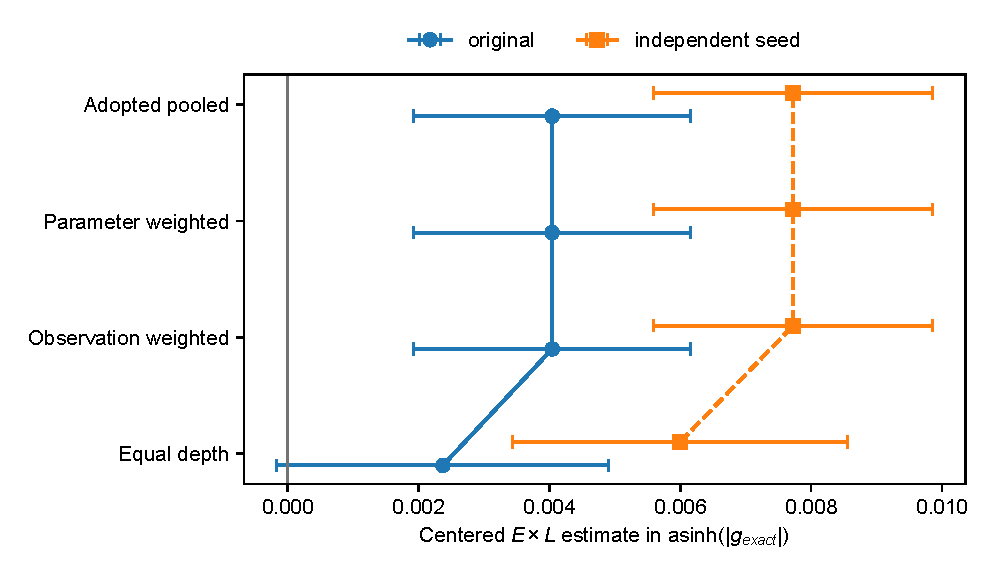
\includegraphics[width=\columnwidth]{fig14_h1_weighting.pdf}
\caption{Post-primary H1 weighting summaries. Equal-depth and observation/matched-parameter weighting answer different questions; the adopted pooled estimate is shown separately. Bars are Wald 95\% intervals, and zero is the reference. Statistical significance is not a criterion for choosing a weighting}
\label{fig:h1-weighting}
\end{figure}

\begin{figure}[t]
\centering
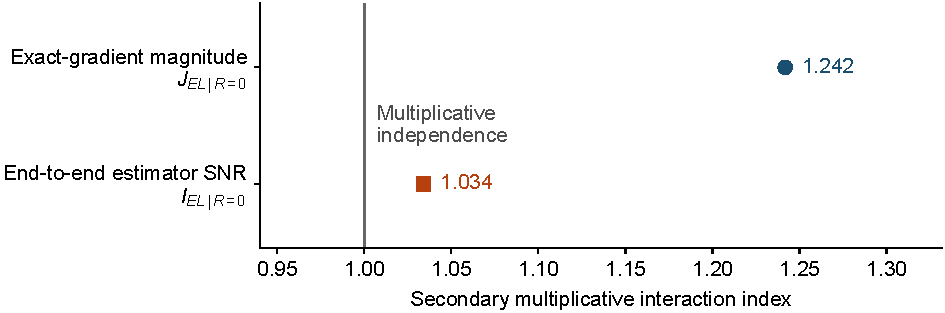
\includegraphics[width=\columnwidth]{fig0_el_primary.pdf}
\caption{Descriptive multiplicative $E\times L$ indices conditional on $R=0$. $I_{EL\mid R=0}$ summarizes end-to-end estimator SNR and $J_{EL\mid R=0}$ exact-gradient magnitude; neither is a centered mixed-model coefficient. The line at one is the multiplicative no-interaction reference}
\label{fig:el-primary}
\end{figure}

\subsection{Finite-shot interaction (H2)}\label{sec:h2-result}

Among positive-variance-eligible end-to-end cells, the corrected centered $E\times L$ coefficient was $0.014338$ (SE $0.005145$, Wald 95\% CI $[0.004255,0.024422]$, raw $p=0.005321$, Holm $p=0.015963$). The model-based Wald/Holm rule rejects H2. Its 1,000-fit nested-bootstrap interval, $[-0.016240,0.045992]$, includes zero. H2 is therefore procedure-sensitive and is not independently corroborated by the nested bootstrap.

\subsection{Residual-related interactions (H3 and H4)}\label{sec:residual-results}

The corrected centered end-to-end $E\times R$ coefficient averaged across $L$ was $-0.011615$ (SE $0.005144$, Wald 95\% CI $[-0.021697,-0.001534]$, raw $p=0.023937$, Holm $p=0.047875$). The model-based rule rejects H3, but its 1,000-fit nested-bootstrap percentile interval $[-0.031375,0.009563]$ includes zero. Matched $R=0$ and $R=1$ gradients are exactly equal at $D=1$ and $D=2$, as required by the inactive shortcut; this structural check passed exactly.

Post-primary end-to-end contrasts explain the averaging: at $L=0$ the estimate was $-0.000958$ (CI $[-0.015251,0.013336]$, $p=0.896$), whereas at $L=1$ it was $-0.022273$ (CI $[-0.036493,-0.008052]$, $p=0.00214$). The corresponding 1,000-fit bootstrap intervals, $[-0.029117,0.024560]$ and $[-0.049490,0.007197]$, include zero. At active depths $D\in\{3,4,6\}$, the L-averaged estimate was $-0.014788$ (CI $[-0.024480,-0.005095]$); $L=0$ remained near zero and $L=1$ was $-0.027449$. Depth-specific averages were $0.006642$, $0.000696$, $-0.026492$, $-0.011553$, and $-0.011255$ at $D=1,2,3,4,6$. Neither model-based ($p=0.545$) nor cluster-robust ($p=0.721$) moderation rejected. Conditional mode reversed direction ($0.006978$, CI $[-0.004745,0.018701]$). Thus H3 is a model-dependent directional signal, objective-specific under end-to-end mode, not a robust or confirmed residual interaction.

The corrected centered $L\times R\times$depth coefficient was $-0.010179$ (SE $0.005362$, Wald 95\% CI $[-0.020688,0.000331]$, raw and Holm $p=0.057658$). Its 1,000-fit nested-bootstrap percentile interval was $[-0.025964,0.005863]$. H4 is not rejected and remains unresolved; this is not evidence of absence.

\begin{table*}[t]
\centering
\footnotesize
\begin{tabularx}{\textwidth}{@{}l p{0.13\textwidth} r l r l >{\raggedright\arraybackslash}X@{}}
\toprule
Hyp. & Estimand & Estimate & Wald 95\% CI & Holm $p$ & Bootstrap 95\% CI & Evidence \\
\midrule
H1 & $E_cL_c$, exact
   & 0.004043
   & \mbox{$[0.001924,\,0.006162]$}
   & 0.000739
   & \mbox{$[0.000473,\,0.007535]$}
   & Both \\
H2 & $E_cL_c$, end-to-end
   & 0.014338
   & \mbox{$[0.004255,\,0.024422]$}
   & 0.015963
   & \mbox{$[-0.016240,\,0.045992]$}
   & Wald only \\
H3 & $E_cR_c$, end-to-end
   & -0.011615
   & \mbox{$[-0.021697,\,-0.001534]$}
   & 0.047875
   & \mbox{$[-0.031375,\,0.009563]$}
   & Wald only \\
H4 & $L_cR_c\times$depth
   & -0.010179
   & \mbox{$[-0.020688,\,0.000331]$}
   & 0.057658
   & \mbox{$[-0.025964,\,0.005863]$}
   & Neither \\
\bottomrule
\end{tabularx}
\caption{Original frozen corrected centered H1--H4 family. Wald intervals and Holm-adjusted $p$-values follow the primary model-based decision rule. The Bootstrap 95\% CI column gives percentile intervals: H1 uses initialization-cluster resampling, whereas H2--H4 use nested initialization-cluster/within-cell replicate resampling with pointwise SNR recomputed before refitting. ``Both'' means that the Wald and bootstrap intervals exclude zero; ``Wald only'' means that the Wald/Holm rule rejects while the bootstrap interval includes zero; and ``Neither'' means that the Wald/Holm rule does not reject and the bootstrap interval includes zero. H1 used 2,000 completed bootstrap fits with zero failures; H2--H4 used exactly 1,000 unique valid fits. These original finite-shot intervals retain component-wise inner resampling; the post-audit vector-preserving intervals are separate in Table~\ref{tab:vector-bootstrap}. Bootstrap iterations are distinct from the 50 top-level initialization clusters.}
\label{tab:confirmatory-summary}
\end{table*}

\begin{figure}[t]
\centering
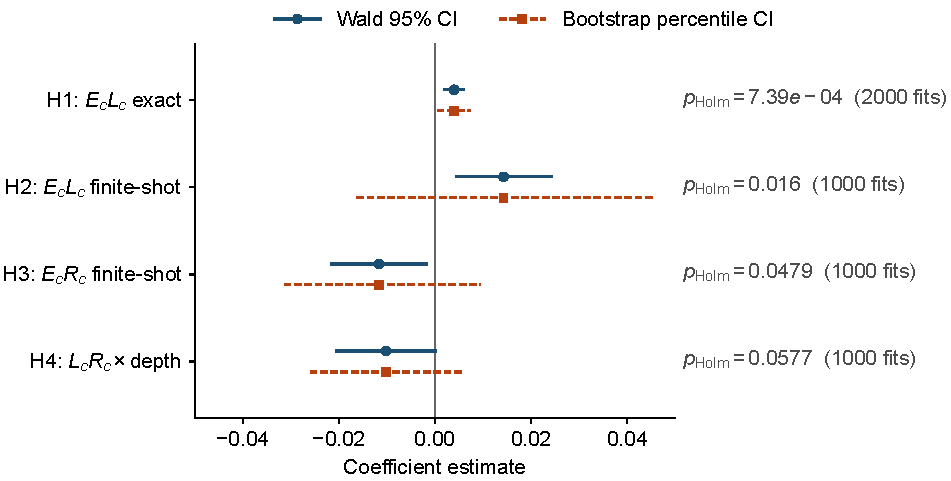
\includegraphics[width=\columnwidth]{fig1_confirmatory_forest.pdf}
\caption{Original frozen primary Wald 95\% intervals and percentile bootstrap intervals for H1--H4, with a zero reference. H1 uses initialization-cluster resampling (2,000 completed fits); H2--H4 use nested initialization-cluster/within-cell replicate resampling (exactly 1,000 unique valid fits). Marker shape and line style distinguish the original interval types without reliance on color; post-audit vector-preserving intervals are reported separately in Table~\ref{tab:vector-bootstrap}}
\label{fig:confirmatory-forest}
\end{figure}

\subsection{Post-audit vector-preserving bootstrap sensitivity}\label{sec:vector-bootstrap-results}
The separate sensitivity completed 1,000 accepted H2--H4 fits from 1,000 attempts, with no failed, rejected, or interrupted draws. Its intervals are shown alongside the original adopted intervals in Table~\ref{tab:vector-bootstrap}. All three still include zero, as do the objective-specific simple H3 contrasts reported in Online Resource~1. Thus this sensitivity did not change zero-crossing classifications and does not corroborate the H2/H3 Wald/Holm rejections or resolve H4. It quantifies the specified resampling-unit comparison on the frozen data rather than establishing bootstrap coverage. Coefficient distributions and interval widths changed; endpoint Monte Carlo uncertainty and the unresolved cross-initialization shot-stream reuse remain relevant. The procedure and sample size were fixed before inspecting the full sensitivity results, without choosing a method for significance.
\begin{table*}[t]\centering\small
\begin{tabular}{lcc}
\toprule
Quantity & Original adopted 95\% interval & Post-audit vector 95\% interval \\
\midrule
H2 & $[-0.016240,0.045992]$ & $[-0.015673,0.045908]$ \\
H3 & $[-0.031375,0.009563]$ & $[-0.032595,0.008511]$ \\
H4 & $[-0.025964,0.005863]$ & $[-0.026397,0.007255]$ \\
\bottomrule
\end{tabular}
\caption{Historical adopted component-wise intervals and the separately labeled post-audit vector-preserving sensitivity, each with 1,000 accepted finite-shot fits. All intervals include zero. Original estimates, Wald/Holm results and the H1 interval remain in Table~\ref{tab:confirmatory-summary}; they are not replaced. These are unadjusted percentile intervals, not a new confirmatory family.}
\label{tab:vector-bootstrap}
\end{table*}

\subsection{Conditional multiplicative indices}

For the original data, $J_{EL\mid R=0}=1.241760$ (bootstrap median $1.238674$, 95\% percentile CI $[1.082210,1.414864]$). At $R=1$, $J_{EL\mid R=1}=1.126633$ (median $1.124329$, CI $[0.991331,1.285152]$), and this interval includes one. New-seed values were $1.163219$ at $R=0$ (median $1.160949$, CI $[1.007100,1.352596]$) and $1.242137$ at $R=1$ (median $1.238157$, CI $[1.049874,1.449258]$). Each bootstrap completed 2,000 iterations with zero failures. These weighting-dependent ratios are descriptive and conditional on $R$; they are not percent improvements and do not measure optimization.

\subsection{Prepared-state metrics and implemented resources}

All bounds, record-key uniqueness, and fidelity--infidelity complementarity checks passed for 4,000 terminal-block prepared-state records at initialization. The count uses unique dataset/initialization/configuration/depth keys after deduplication across shot budgets; physical quantum-state uniqueness was not independently established. Cell mean fidelity ranged approximately $0.0338$--$0.0817$ in the original data and $0.0322$--$0.0962$ in the independent-seed data; normalized prepared-state energy means ranged $0.4631$--$0.5529$ and $0.4561$--$0.5537$, respectively. The ranges overlap strongly and show no conspicuous seed-unstable separation descriptively. They do not demonstrate training success or a causal relationship between gradient magnitude and task quality.

All 320 resource-design rows conserve nominal implemented $B$, with no negative allocations or zero-shot production jobs. All 1,833 zero-variance cells joined to complete resource records. At $D=6$, the extremes are 48 jobs for conditional/global and 61 for end-to-end/local, a 27.08\% increase. This is a simulator job-count comparison, not a matched physical-resource or wall-clock claim.

\subsection{Implementation checks}\label{sec:results-robustness}

Black-box finite differences checked 224 quantum-parameter derivatives across 16 cases at $D=1$ and $D=6$, configurations 1, 2, 3, and 5, and steps $10^{-3},10^{-4},10^{-5}$. At $10^{-5}$, the maximum relative error was $1.27\times10^{-5}$ overall and $9.77\times10^{-7}$ among 214 gradients with magnitude at least $10^{-5}$; four near-zero gradients exceeded the relative tolerance but had small absolute errors (the maximum over all 224 derivatives at step $10^{-5}$ was below $1.62\times10^{-11}$), with no sign or order-of-magnitude failures. Centered and direct models were verified as exact reparameterizations, primary and diagnostic model entry points were guarded against mode pooling, and frozen outputs passed deterministic regeneration and manifest-integrity tests. The adopted H2--H4 fit converged with L-BFGS, was nonsingular, emitted one boundary warning, and agreed with a forced BFGS refit within the verified direct-coded coefficient error bounds given in Methods; residual heteroscedasticity and heavy tails remain covariance caveats. Online Resource 1 reports complete diagnostics.

\section{Discussion}

\subsection{Principal findings}

H1 provides the strongest cross-procedure evidence. Its positive centered exact-gradient direction appears in both seed sets and both initialization-cluster bootstrap intervals exclude zero. Table~\ref{tab:h1-marginal-effects} shows that the pair-restricted schedule has a larger adjusted effect under TFIM energy than under global infidelity, while the corresponding differences between back-transformed adjusted locations remain modest in absolute magnitude. Its magnitude and depth profile nevertheless remain uncertain: the seed-set point estimates differ, the original equal-depth interval includes zero while its observation-weighted interval does not, and the original moderation conclusion depends on covariance estimator.

H2 and H3 require a different interpretation. Both meet the primary model-based Wald/Holm rejection rule, yet their nested-bootstrap intervals include zero. H2 is additionally conditional on objective-linked positive-variance eligibility. H3's end-to-end direction is concentrated in the energy-objective condition, reverses under conditional mode, and is not supported by cluster-robust depth moderation. H4 is not rejected and remains unresolved rather than proved absent. Post-primary analyses therefore indicate that H1's pooled positive direction is reproducible across seed sets, but its magnitude and depth profile are uncertain; H2 and H3 remain procedure-sensitive because their Wald/Holm rejections are not corroborated by the corresponding nested-bootstrap intervals. The separately labeled post-audit whole-vector sensitivity retains zero-spanning H2--H4 and simple H3 intervals, so it does not change these classifications. This is evidence about that specified sensitivity, not proof of nominal coverage or a repair of cross-cluster seed reuse.

Conditional $J$ ratios provide descriptive multiplicative summaries, with positive above-reference patterns in several dataset--residual combinations. They are weighting-dependent, conditional on $R$, and not algebraic equivalents of centered mixed-model coefficients. Prepared-state metrics likewise describe initialization states only; they neither demonstrate training success nor establish that larger initial gradients causally improve energy or fidelity. Resource accounting applies to the implemented simulator protocol: total $B$ is conserved, but job counts and shots per job differ, and no physical-resource or hardware-cost equality follows.

\subsection{Interpretation and relation to prior work}

Local objectives can improve gradient scaling under specified circuit-depth assumptions, while excessive random entanglement can suppress gradients \cite{cerezo2021costfunction,ortizmarrero2021entanglement,patti2021entanglement}. The present result connects these observations statistically: in this four-qubit reset-based architecture, the modeled objective contrast is larger under the restricted CNOT schedule than expected from the two marginal effects on the transformed response scale. This non-additivity is compatible with theoretical accounts that treat architecture, state structure, and observable support as coupled determinants of loss concentration \cite{ragone2024lie}, but it neither identifies a physical mechanism nor tests asymptotic barren-plateau scaling.

The $L$ factor also changes more than measurement locality. Normalized TFIM energy and global infidelity differ in spectral weighting, observable decomposition, circuit count, and landscape geometry. Likewise, the $E$ factor is one specific four-CNOT schedule and the $R$ factor is one fixed-gain shortcut between reset blocks. The observed coefficients should therefore be interpreted as interactions among these implemented contrasts, not universal laws about low entanglement, local costs, or residual quantum networks.

The results concern matched initial parameter points rather than complete optimization trajectories. A resolvable initial gradient is neither necessary nor sufficient for convergence, and residual architectures evaluated over full training trajectories address a different estimand \cite{anschuetz2022traps,grant2019identity,skolik2021layerwise,kashif2024resqnets}. The unstable residual-interaction evidence here does not contradict optimization results in other architectures.

\subsection{Implications for QML evaluation}

The observed interaction illustrates why gradient-resolvability interventions can warrant joint rather than exclusively marginal evaluation. A factorial design can reveal pairwise non-additivity and moderation without implying that a fully combined configuration is universally preferable. Future benchmarks should test both whether interventions interact and whether those interactions vary with architecture-size variables.

Finite-shot metrics also require operational definitions that are treated as part of the experiment. Matching total shots does not match per-circuit precision; re-estimating intermediate features changes bias and sign reliability; and plug-in ratios can generate factor-dependent eligibility when estimated variance is zero. Eligibility rules, estimator modes, seed derivation, and regression guards should be specified and tested as carefully as the statistical formula itself.

\subsection{Limitations and priorities for follow-up}\label{sec:limitations}

The experiment covers four qubits, one open-boundary TFIM task, one reset-per-block architecture, one implementation of each intervention, one initialization family, and 50 top-level initialization clusters per dataset where applicable. Exact-state and abstract shot simulation omit hardware noise, readout and calibration models, and wall-clock behavior. There are no optimization trajectories; task metrics are terminal-block prepared-state quantities at initialization only.

Finite-replicate zero-variance selection is tied to $L$. Increasing parameter count with depth induces observation/parameter weighting, and some depth conclusions are covariance-sensitive. H2 and H3 disagree across inference procedures, while H3 also disagrees across estimator modes. Conditional $J$ quantities are weighting-dependent descriptive summaries. Ambiguity in the published protocol regarding reset semantics and factor coding remains a provenance limitation. No matched physical-resource claim is available because circuits, jobs, shots per circuit, gates, calibration, readout, noise, and time were not jointly matched. The original inner bootstrap lost within-vector dependence; its historical intervals are retained alongside the post-audit vector-preserving assessment. The latter retains repeated shot streams across some initialization clusters. Their inferential effect has not been isolated. Independent prospective initialization-pilot input and the original sample-size decision chronology are unverified; the archived initialization-count calculation is retrospective. Endpoint Monte Carlo uncertainty, including the retained singularity flag in one converged post-audit draw, further limits interpretation.

Follow-up work would require prospectively specified additional datasets, continuous-state architectural controls, optimization trajectories, and hardware-noise experiments; none is inferred from the present initialization analysis.

\section{Conclusion}\label{sec:conclusion}

In this matched four-qubit factorial experiment, the principal empirical finding is a positive CNOT-schedule $\times$ objective interaction in transformed exact-gradient magnitude. The adopted parameter-weighted coefficient is supported by model-based and initialization-cluster bootstrap inference; an independent-seed analysis corroborates the positive direction, though coefficient magnitude and block-count profile remain uncertain. The finite-shot $E\times L$ and $E\times R$ interactions meet the primary Wald/Holm criterion but lack nested-bootstrap corroboration, and the $L\times R$-by-block-count interaction is unresolved. The post-audit, 1,000-fit vector-preserving sensitivity also leaves the finite-shot intervals spanning zero; it supplements rather than replaces the original primary family.

These differences underscore why exact-gradient landscape structure, finite-shot estimator SNR, estimator bias, and gradient sign reliability should not be treated as interchangeable indicators of trainability. The study provides a self-contained, measurement-aware factorial benchmark for particular circuit, objective, and residual implementations. It motivates interaction-focused QNN comparisons without establishing optimization improvement, asymptotic barren-plateau mitigation, or matched hardware-resource advantages.

\backmatter

\section*{Acknowledgements}

\textbf{Generative-AI assistance.} Anthropic Claude and OpenAI Codex were used during 2026 for literature-search planning, clarification of technical concepts, implementation and verification scripting, consistency checking, and feedback on author-written prose. These systems were not treated as authors or evidentiary sources. The author independently inspected the cited literature, executed and reviewed the code, verified the numerical outputs, and accepts responsibility for every claim and analysis decision.

\section*{Statements and Declarations}

\bmhead{Funding} No external funding was received.

\bmhead{Competing interests} The author declares no financial or non-financial competing interests.

\bmhead{Ethics approval} Not applicable. This study used computational simulations and did not involve human participants, human data, animals, or biological materials.

\bmhead{Consent to participate} Not applicable.

\bmhead{Consent for publication} Not applicable.

\bmhead{Author contributions} Brandon Shen conceived the study, implemented the simulation and analysis pipeline, conducted the experiments and verification analyses, interpreted the results, prepared the figures, and wrote and revised the manuscript.

\bmhead{Data availability} The machine-readable numerical source is \texttt{results/final\_submission\_v1/manifest.json}. The numerical-results freeze is \nolinkurl{submission-numerical-results-freeze-v1}. The accompanying OSF project is available at \href{https://doi.org/10.17605/OSF.IO/THV6G}{\nolinkurl{https://doi.org/10.17605/OSF.IO/THV6G}}. The preserved pre-remediation manuscript-facing repository snapshot is the release \href{https://github.com/Brandon-Shen/few-qubit-qnn-snr/releases/tag/sndc-submission-v1}{\texttt{sndc-submission-v1}}. Files under \path{results/superseded/}, \path{results/superseded_pooled/}, and other explicitly superseded directories are historical material and must not be read as current primary conclusions. The historical release's copy of \texttt{MANUSCRIPT\_COMMIT.txt} records the exact substantive commit against which the manuscript sources, numerical values, tables, figures, and documentation were finalized.

\paragraph{Separate post-audit provenance records.}
The original numerical freeze and both original reference inventories are preserved. Five standalone component hashes and both inventories' byte counts describe CRLF versions of current LF-normalized text artifacts; the manifest's component hashes describe the LF content. This is a line-ending metadata discrepancy, not a demonstrated change of scientific numbers. Verified proposed correction records, including canonical-LF byte counts, are in \path{verification/independent_audit/remediation/stage4_20261122_provenance_descriptives/provenance_correction_metadata.json}. Point estimates and Wald/Holm quantities come from \path{results/primary_corrected/effect_coded/corrected_confirmatory_hypotheses.csv}; adopted bootstrap endpoints come from the separate \path{results/primary_corrected/effect_coded/corrected_bootstrap_intervals_current_draws.csv}. The row-keyed \path{verification/independent_audit/remediation/stage4_20261122_provenance_descriptives/bootstrap_interval_provenance_overlay.json} records both paths/hashes, draw sources, and input roles without rewriting frozen fields. Post-audit vector-preserving coefficients and intervals are separate evidence under \path{verification/independent_audit/remediation/stage3_20261121_full_vector_sensitivity/analyses/finalization_0000/}. The proposed repository release \nolinkurl{sndqs-submission-v1} is unpublished. The release evidence index is \path{submission/sndqs-submission-v1/EVIDENCE_INDEX.md}.

\bmhead{Code availability} The preserved pre-remediation, versioned manuscript, code, documentation, verification scripts, and submission-facing repository state are available in the \href{https://github.com/Brandon-Shen/few-qubit-qnn-snr/releases/tag/sndc-submission-v1}{\texttt{sndc-submission-v1}} release. The associated OSF project is available at \href{https://doi.org/10.17605/OSF.IO/THV6G}{\nolinkurl{https://doi.org/10.17605/OSF.IO/THV6G}}. The GitHub release is distinct from the numerical-results freeze identified above. The repository contains the simulation and gradient code, mixed-model and multiplicity analyses, bootstrap implementations, robustness analyses, figure scripts, and regression tests; The proposed release \nolinkurl{sndqs-submission-v1} will identify the remediated source and code state. It is unpublished.

\bmhead{Materials availability} Not applicable.

\bmhead{Software and reproducibility information} The recorded production environment was CPython 3.12.10 on Windows 11, with PennyLane 0.45.1, NumPy 2.5.1, pandas 3.0.3, SciPy 1.18.0, statsmodels 0.14.6, PyArrow 25.0.0, Matplotlib 3.11.0, and PyYAML 6.0.3. These versions are supported by \path{results/production_confirmatory/run_manifest.json}, the numerical-freeze environment record, and \path{requirements-lock.txt}. The latter pins direct dependencies and development extras only; a complete original transitive dependency lock has not been recovered, and a later installed-package snapshot is not an original full lock. Shot streams use deterministic SHA-256-derived seeds with the finite-space reuse disclosed in Section~\ref{sec:shot-stream-audit}. Original and post-audit bootstrap provenance are documented separately in Online Resource~1.

\bmhead{Supplementary information} Online Resource 1 contains additional estimator-eligibility analyses, model and influence diagnostics, the documented estimator-mode correction, bootstrap and depth-sensitivity results, and a reproducibility index. The supplementary file is provided as \texttt{ESM\_1.pdf}.

\bibliography{references}

\end{document}